
\documentclass[10pt,twocolumn]{article}

\usepackage[margin=0.72in,columnsep=0.24in]{geometry}
\usepackage{fontspec}
\setmainfont{DejaVu Sans}
\setsansfont{DejaVu Sans}
\newfontfamily\cjkfont{WenQuanYi Micro Hei}
\XeTeXlinebreaklocale "zh"
\XeTeXlinebreakskip=0pt plus 1pt
\usepackage{graphicx}
\usepackage{booktabs}
\usepackage{amsmath,amssymb}
\usepackage{multirow}
\usepackage{xcolor}
\usepackage{hyperref}
\usepackage{caption}
\usepackage{subcaption}
\usepackage{enumitem}
\usepackage{titlesec}
\usepackage{microtype}

\definecolor{cvblue}{HTML}{2563EB}
\hypersetup{colorlinks=true,linkcolor=cvblue,citecolor=cvblue,urlcolor=cvblue}
\captionsetup{font=small,labelfont=bf}
\setlist[itemize]{leftmargin=1.2em,itemsep=0.1em,topsep=0.2em}
\titleformat{\section}{\large\bfseries}{\thesection}{0.55em}{}
\titleformat{\subsection}{\normalsize\bfseries}{\thesubsection}{0.5em}{}

\title{\vspace{-1.0em}\bfseries FisheyeMotion: {\cjkfont 面向鱼眼视频运动区域抽象的多源深度证据融合与双路线评估}}
\author{{\cjkfont 2354265 庄嘉瀚 \quad 2351745 张巍瀚}\\{\cjkfont 同济大学}}
\date{}

\begin{document}
\maketitle
\vspace{-1.1em}

\begin{abstract}
{\cjkfont 鱼眼视频以大视场覆盖换取强非线性投影畸变，使同一三维运动在图像中心与边缘呈现显著不同的尺度、边界和光流统计。本文提出} \textbf{FisheyeMotion}{\cjkfont ，一个面向相邻鱼眼帧运动区域抽象与短时目标跟踪的} GPU {\cjkfont 深度学习系统。系统融合} RAFT {\cjkfont 光流、}YOLO26-seg {\cjkfont 实例先验、}DINOv2 {\cjkfont 语义变化、边界提示、鱼眼几何编码、监督式} FisheyeMotionNet{\cjkfont 、测试时增强不确定性融合与} SAM2.1 {\cjkfont 掩膜细化。针对课程要求中的两种技术路线，我们分别实现原始鱼眼域处理与校正域处理，并将校正域预测反投影回鱼眼域进行公平评估。实验在} 130 {\cjkfont 个有效样本上完成训练、消融、区域评估和路线对比；测试集包含} 19 {\cjkfont 个样本。结果显示，原始鱼眼域完整模型取得} IoU 0.2959{\cjkfont 、}Precision 0.3352{\cjkfont 、}Recall 0.5941{\cjkfont 、}F1 0.3758{\cjkfont ，显著优于} FrameDiff{\cjkfont 、}Farneback {\cjkfont 和} RAFT-only{\cjkfont ，并在边缘区域达到} F1 0.2916{\cjkfont 。与之相比，校正路线完整模型} F1 {\cjkfont 为} 0.0883{\cjkfont ，说明在本数据规模和当前反投影误差下，保持原始鱼眼域并显式注入几何先验比前置校正更可靠。}
\end{abstract}

\section{{\cjkfont 引言}}
{\cjkfont 运动区域抽象是视频理解、智能交通监控和移动机器人感知中的基础任务。与针孔相机相比，鱼眼相机能够覆盖更宽视场，但其径向畸变会改变目标形状、像素速度和局部纹理统计。中心区域目标通常具备较稳定的外观和边界，而边缘区域目标被压缩或拉伸，光流幅值与真实运动不再简单对应，运动边界也更容易与静态结构、车体反光和镜头遮挡混淆。}

{\cjkfont 传统帧差、}Farneback {\cjkfont 光流和单一深度光流阈值都难以处理上述问题。仅依赖实例分割也不充分，因为检测模型能定位物体，却不能判断物体是否相对场景发生运动。本文的核心观点是：鱼眼运动分割需要联合建模运动、实例、语义、边界和投影几何，而不是把任务退化为某一种证据的阈值化。}

{\cjkfont 本文贡献如下：}
\begin{itemize}
  \item {\cjkfont 构建完整} GPU {\cjkfont 实验流程，覆盖数据校验、}RAFT/YOLO/DINO {\cjkfont 特征缓存、监督训练、}SAM2.1 {\cjkfont 细化、区域评估、短时跟踪和可复现脚本。}
  \item {\cjkfont 提出多源证据融合的} FisheyeMotionNet{\cjkfont ，将} RGB pair{\cjkfont 、帧差、深度光流、实例} mask{\cjkfont 、语义变化、边界提示和鱼眼几何编码统一到监督分割框架。}
  \item {\cjkfont 实现原始鱼眼域与校正域两条路线，并在相同鱼眼} GT {\cjkfont 上公平比较，揭示当前任务中前置校正会显著损害最终掩膜质量。}
\end{itemize}

\begin{figure*}[t]
  \centering
  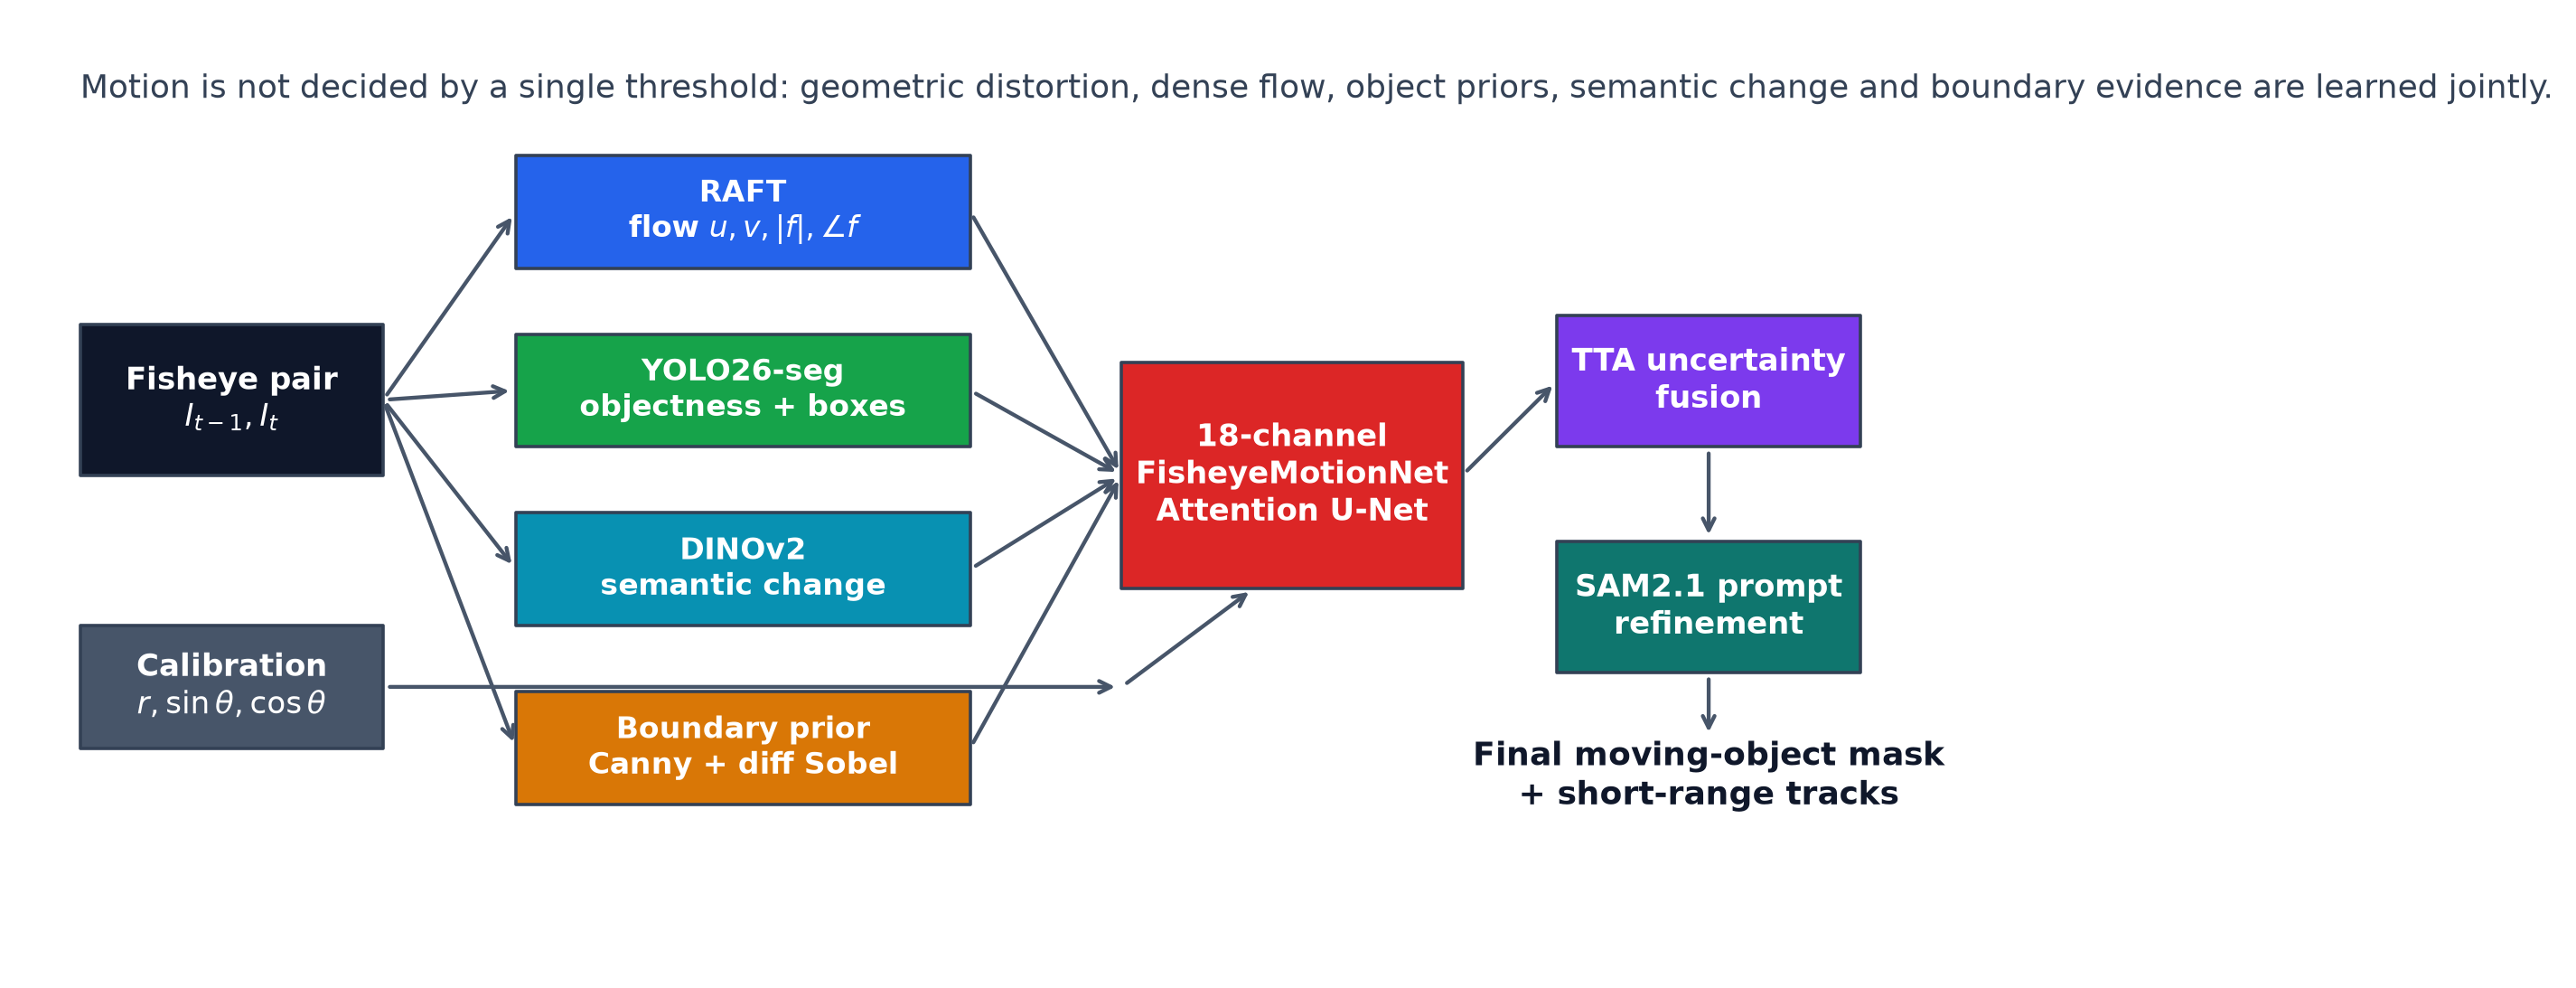
\includegraphics[width=\textwidth]{../figures/architecture_graph.png}
  \caption{\textbf{FisheyeMotion {\cjkfont 总体架构。}} {\cjkfont 系统联合} RAFT {\cjkfont 光流、}YOLO {\cjkfont 实例先验、}DINOv2 {\cjkfont 语义变化、边界提示和鱼眼几何图，经} FisheyeMotionNet {\cjkfont 预测运动概率，再通过不确定性融合与} SAM2.1 prompt refinement {\cjkfont 生成最终运动掩膜和短时轨迹。}}
  \label{fig:architecture}
\end{figure*}

\section{{\cjkfont 相关工作}}
\textbf{{\cjkfont 光流估计。}} RAFT~\cite{teed2020raft} {\cjkfont 通过} all-pairs correlation volume {\cjkfont 和循环更新模块显著提高稠密光流质量，}SEA-RAFT~\cite{wang2024searaft} {\cjkfont 进一步探索效率与精度平衡。本文使用} RAFT large {\cjkfont 作为强运动底座，但避免直接阈值化光流，而是将其作为可学习输入和短时传播线索。}

\textbf{{\cjkfont 提示分割与视频分割。}} SAM2~\cite{ravi2024sam2} {\cjkfont 将} promptable segmentation {\cjkfont 扩展到图像和视频，}Cutie~\cite{cheng2024cutie} {\cjkfont 则强调对象记忆在视频目标分割中的作用。本文任务主要由相邻帧} pair {\cjkfont 构成，因此不追求长时记忆建模，而是利用} SAM2.1 {\cjkfont 对高置信运动提示进行边界} densification{\cjkfont 。}

\textbf{{\cjkfont 自监督语义表征。}} DINOv2~\cite{oquab2023dinov2} {\cjkfont 的} patch token {\cjkfont 具有良好的类别无关语义聚合能力。受} Segment Any Motion~\cite{li2025segmentanymotion} {\cjkfont 将运动线索、}DINO {\cjkfont 表征与} SAM {\cjkfont 掩膜组合的思想启发，我们将} DINOv2 semantic saliency {\cjkfont 和前后帧} semantic change {\cjkfont 作为小样本运动分割的补充证据。}

\section{{\cjkfont 方法}}
\subsection{{\cjkfont 鱼眼几何编码}}
{\cjkfont 给定每个样本的标定} JSON{\cjkfont ，我们根据主点} $(c_x,c_y)$ {\cjkfont 生成归一化半径与方向编码：}
\begin{equation}
  r(x,y)=\frac{\sqrt{(x-c_x)^2+(y-c_y)^2}}{r_{\max}},\quad g(x,y)=[r,\sin\theta,\cos\theta].
\end{equation}
{\cjkfont 该几何图不直接校正图像，而是作为网络输入，让模型学习不同半径处运动证据的可信度。评估时按} $r<0.35${\cjkfont 、}$0.35\le r<0.70${\cjkfont 、}$r\ge0.70$ {\cjkfont 划分中心、中间和边缘区域。}

\subsection{{\cjkfont 多源证据提取}}
{\cjkfont 对每个相邻帧} pair{\cjkfont ，系统缓存以下证据：}RAFT {\cjkfont 输出} $u,v,|f|,\angle f${\cjkfont ；}YOLO26-seg {\cjkfont 输出实例} objectness mask{\cjkfont ；}DINOv2 {\cjkfont 输出当前帧} saliency {\cjkfont 和前后帧} semantic change{\cjkfont ；边界提示由} Canny {\cjkfont 边缘与帧差} Sobel {\cjkfont 梯度组合得到。真实缓存证据如图}~\ref{fig:evidence} {\cjkfont 所示。}

\begin{figure*}[t]
  \centering
  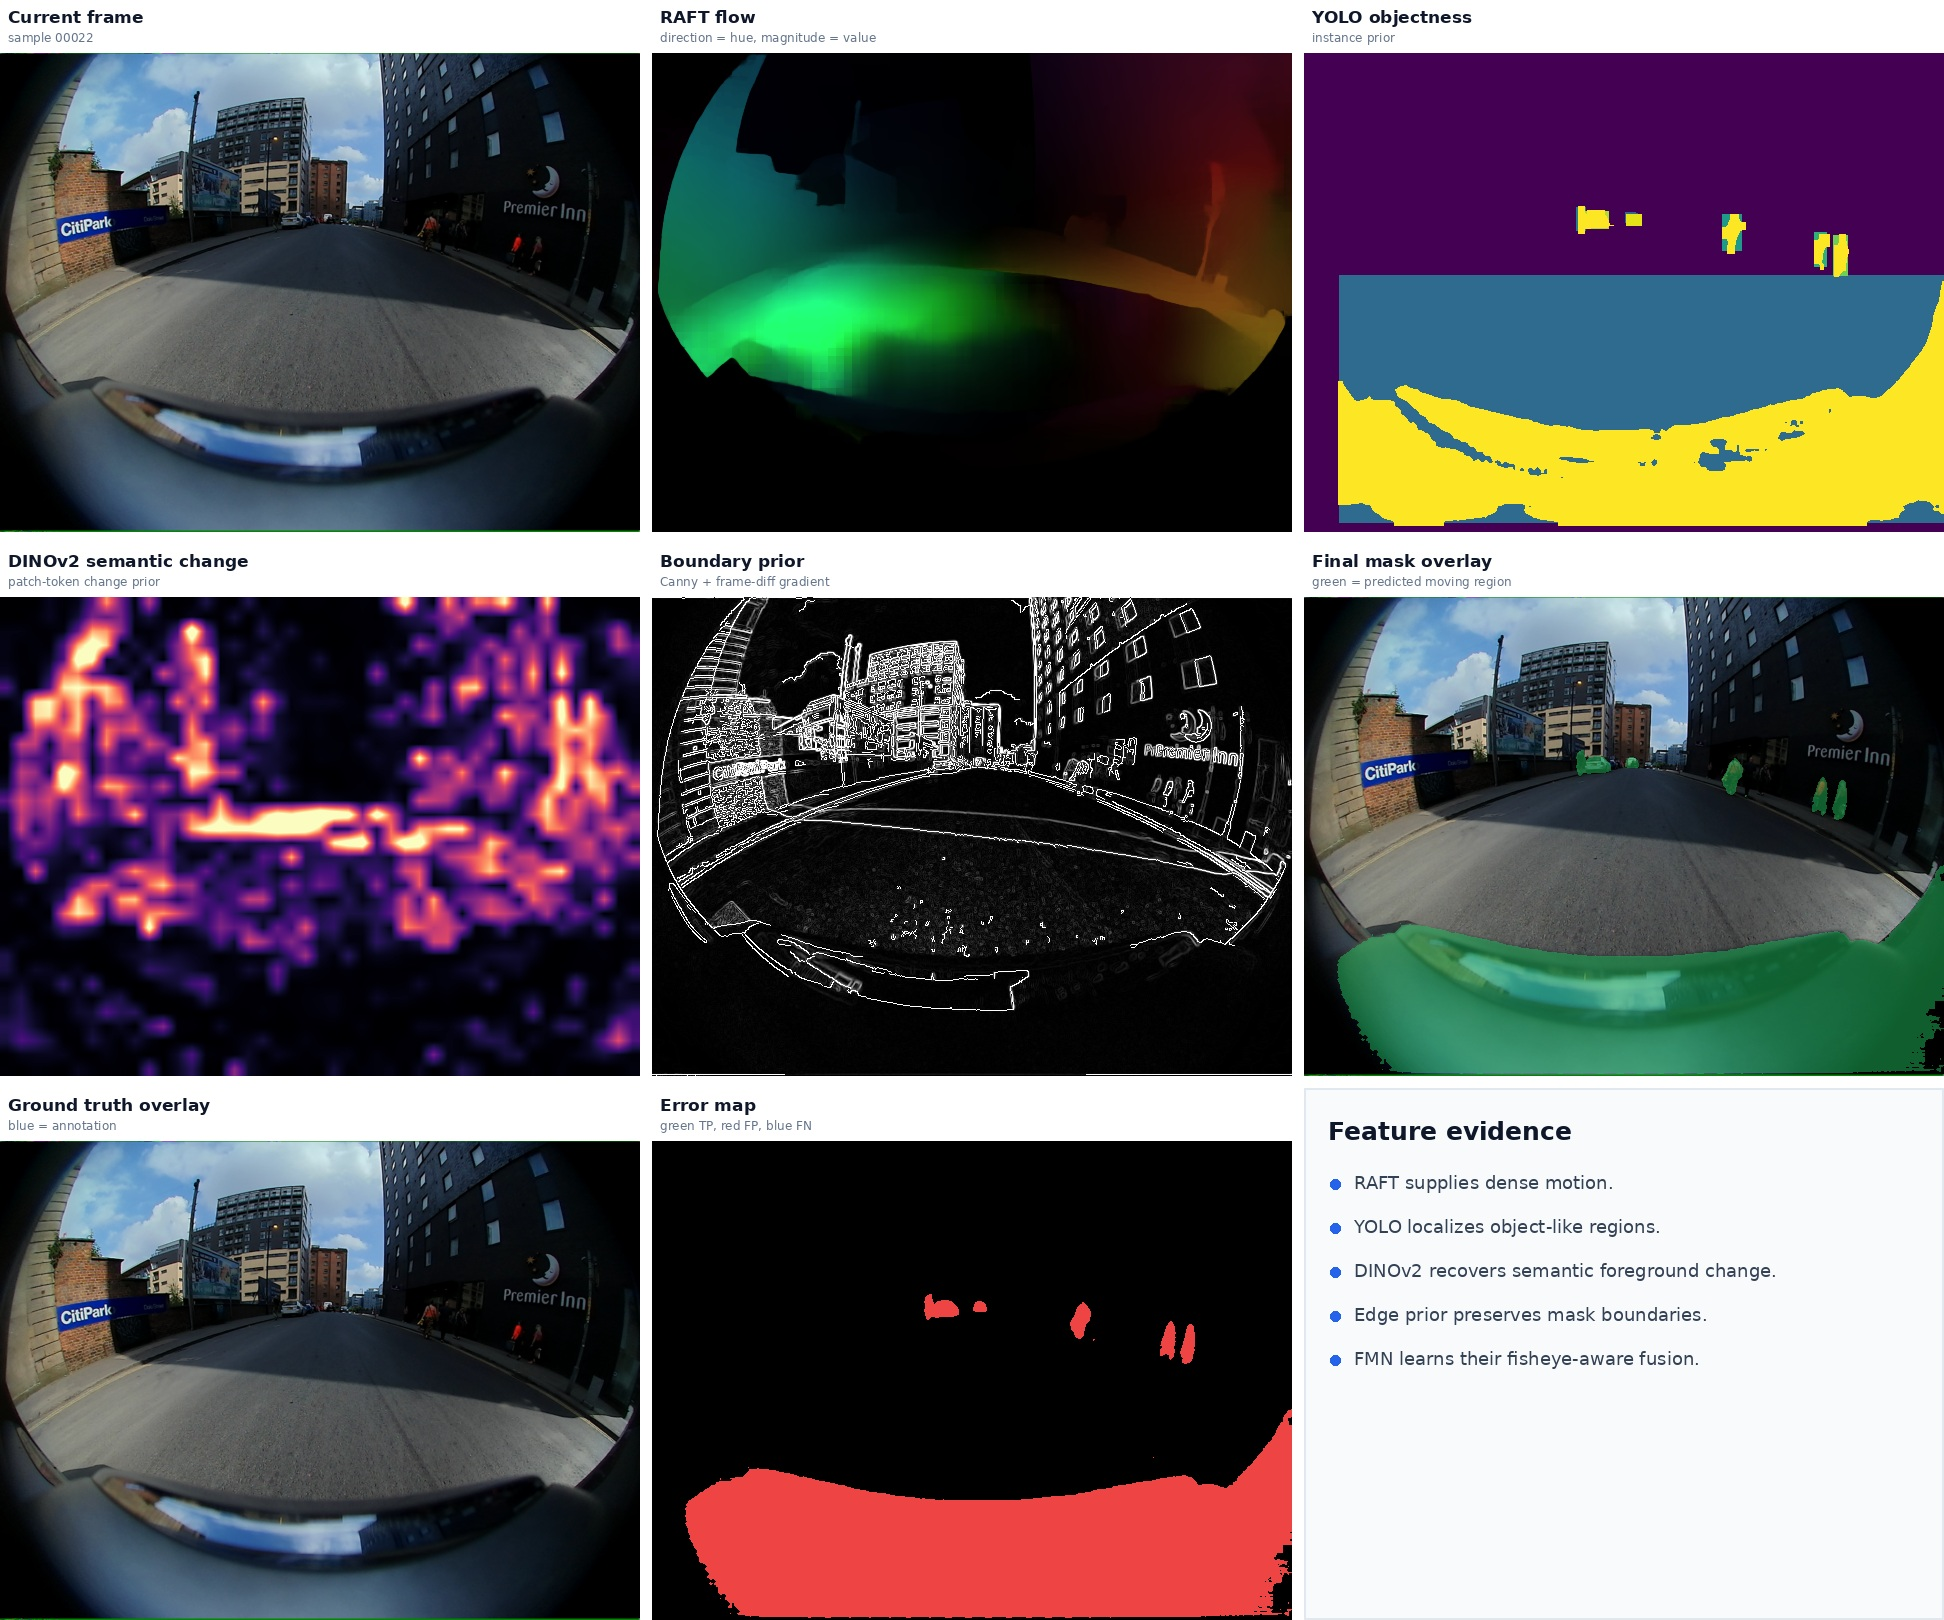
\includegraphics[width=\textwidth]{../figures/feature_evidence_panel.jpg}
  \caption{\textbf{{\cjkfont 真实模型证据面板。}} {\cjkfont 该图展示最终模型实际使用的当前帧、}RAFT {\cjkfont 光流、}YOLO objectness{\cjkfont 、}DINOv2 semantic change{\cjkfont 、边界先验、最终预测、}GT {\cjkfont 与误差图。红色为} FP{\cjkfont ，蓝色为} FN{\cjkfont ，绿色为} TP{\cjkfont 。}}
  \label{fig:evidence}
\end{figure*}

\subsection{FisheyeMotionNet}
FisheyeMotionNet {\cjkfont 是一个轻量} Attention U-Net {\cjkfont 风格分割网络，输入为：}
\begin{equation}
\begin{split}
X = [&I_{t-1}^{rgb}, I_t^{rgb}, |I_t-I_{t-1}|, f_{RAFT}, M_{YOLO},\\
&P_{DINO}^{sal}, P_{DINO}^{chg}, P_{edge}, g(x,y)].
\end{split}
\end{equation}
{\cjkfont 训练目标由边界加权} BCE{\cjkfont 、}Dice loss {\cjkfont 和} boundary loss {\cjkfont 组成：}
\begin{equation}
  \mathcal{L}=\mathcal{L}_{BCE}^{w}+\lambda_d\mathcal{L}_{Dice}+\lambda_b\mathcal{L}_{Boundary}.
\end{equation}
{\cjkfont 边界权重由} GT {\cjkfont 膨胀边缘生成，用于缓解小目标和细边界在背景中被淹没的问题。}

\subsection{{\cjkfont 不确定性融合与} SAM2.1 {\cjkfont 细化}}
{\cjkfont 推理阶段使用原图和水平翻转两路} TTA{\cjkfont ，预测均值作为} $P_{net}${\cjkfont ，标准差作为} epistemic uncertainty $U${\cjkfont 。融合分数定义为：}
\begin{equation}
S=w_nP_{net}+w_fP_{flow}+w_yP_{yolo}+w_dP_{dino}+w_eP_{edge}-w_uU.
\end{equation}
{\cjkfont 高置信点、运动连通域框和} YOLO {\cjkfont 框共同组成} SAM2.1 prompts{\cjkfont 。该设计使} SAM2.1 {\cjkfont 主要负责边界细化，运动属性仍由多源证据和监督网络决定。}

\section{{\cjkfont 实验设置}}
{\cjkfont 实验使用课程提供的鱼眼图像数据集，样本由当前帧、前一帧、}GT {\cjkfont 掩膜和鱼眼标定文件组成。共验证} 130 {\cjkfont 个完整样本，图像原始尺寸为} $1280\times966${\cjkfont 。训练}/{\cjkfont 验证}/{\cjkfont 测试比例为} 70/15/15{\cjkfont ，测试集} 19 {\cjkfont 个样本。所有深度模块均强制使用} GPU{\cjkfont ；实验环境为} NVIDIA GeForce RTX 3060 Laptop GPU{\cjkfont ，}PyTorch 2.11.0+cu128{\cjkfont 。实验流程可由以下命令复现：}
\begin{center}
\small\texttt{bash scripts/run\_full\_pipeline.sh}
\end{center}
{\cjkfont 该脚本依次执行数据校验、鱼眼域训练评估、校正域训练评估、消融、区域评估和路线对比。}

\section{{\cjkfont 结果}}
\subsection{{\cjkfont 主结果}}
\begin{table}[t]
\centering
\caption{{\cjkfont 原始鱼眼域测试集主结果。表中数值为固定测试集上的平均指标。}}
\label{tab:fisheye-main}
\resizebox{\columnwidth}{!}{
\begin{tabular}{lcccc}
\toprule
Method & IoU & Prec. & Rec. & F1\\
\midrule
FrameDiff & 0.0376 & 0.0534 & 0.4058 & 0.0658\\
Farneback & 0.0147 & 0.0298 & 0.1072 & 0.0275\\
RAFT-only & 0.0264 & 0.0512 & 0.1150 & 0.0462\\
YOLO-only & 0.2384 & 0.2588 & 0.5933 & 0.3292\\
FisheyeMotionNet & 0.2718 & 0.3549 & 0.4504 & 0.3589\\
UncertaintyFusion & 0.2727 & 0.3595 & 0.4433 & 0.3596\\
\textbf{Full} & \textbf{0.2959} & 0.3352 & \textbf{0.5941} & \textbf{0.3758}\\
\bottomrule
\end{tabular}}
\end{table}

{\cjkfont 表}~\ref{tab:fisheye-main} {\cjkfont 表明，传统方法在鱼眼视频中显著受限。}FrameDiff {\cjkfont 具有较高召回但} precision {\cjkfont 极低，说明其将光照变化、静态边缘和反光区域误判为运动。}Farneback {\cjkfont 与} RAFT-only {\cjkfont 的} F1 {\cjkfont 均低于} 0.05{\cjkfont ，说明仅依赖光流幅值不足以解决鱼眼畸变和实例语义混淆。}YOLO-only F1 {\cjkfont 达到} 0.3292{\cjkfont ，证明实例先验很关键，但它缺少运动属性判断。完整模型在保持高召回的同时提升综合} F1 {\cjkfont 至} 0.3758{\cjkfont 。}

\begin{figure}[t]
  \centering
  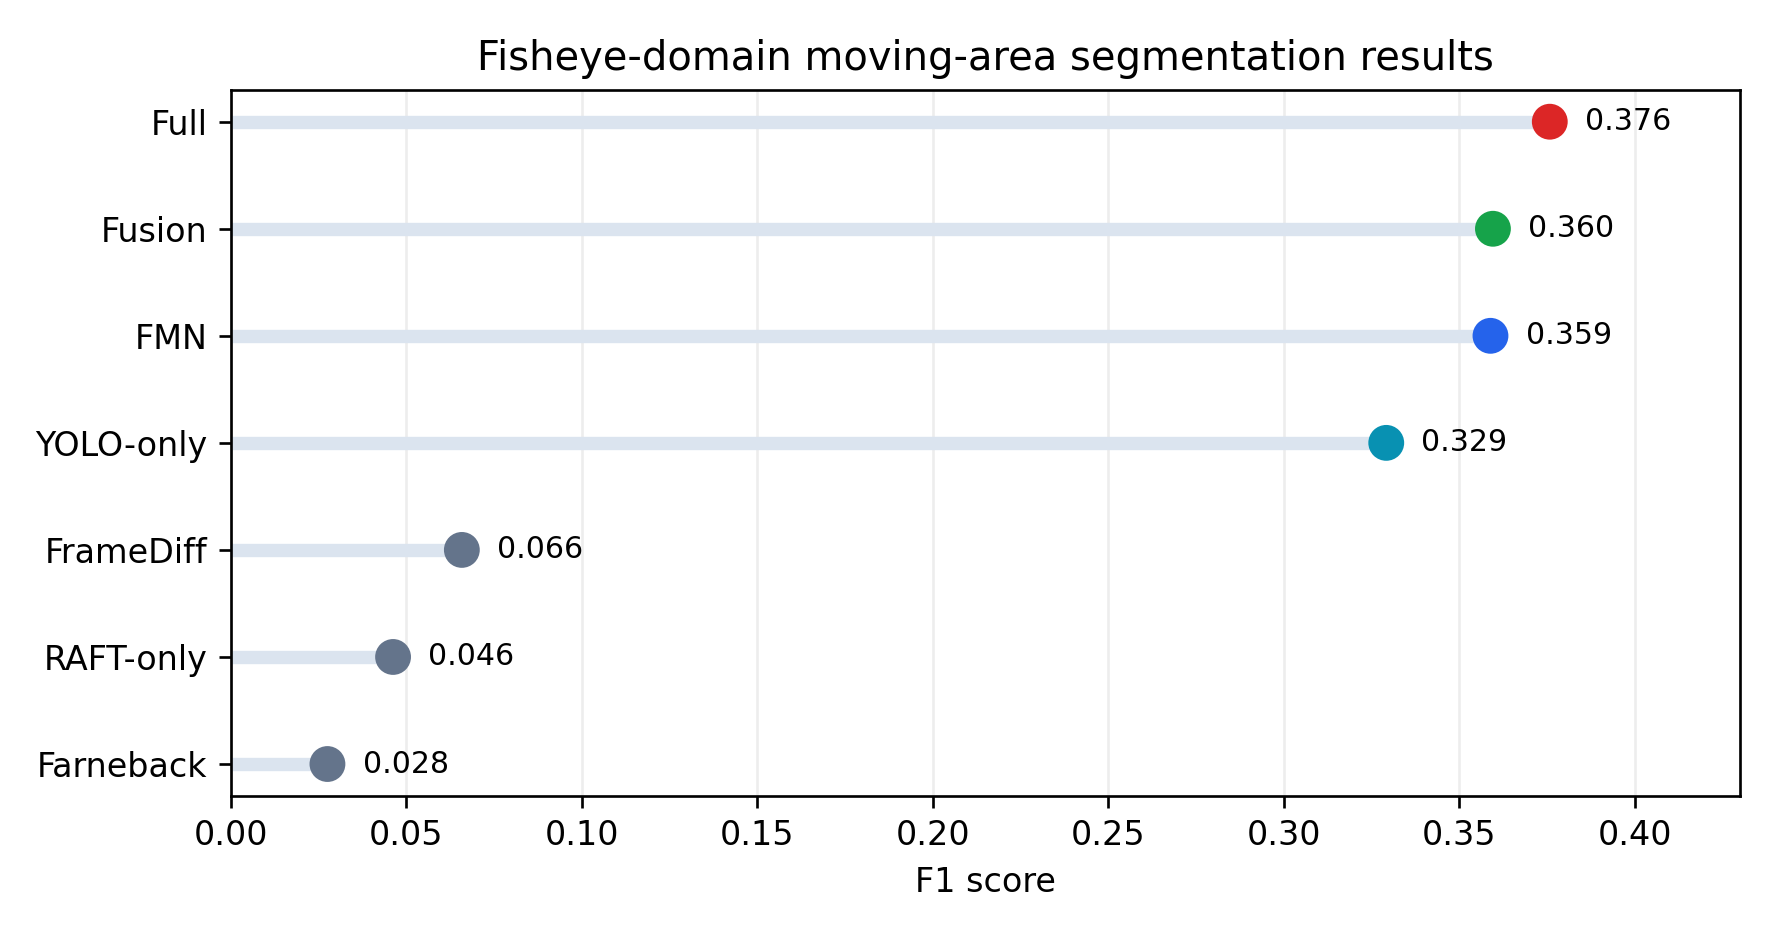
\includegraphics[width=\columnwidth]{../figures/method_ranking.png}
  \caption{\textbf{{\cjkfont 鱼眼域方法} F1 {\cjkfont 对比。}} {\cjkfont 深度融合方法显著优于传统帧差、}Farneback {\cjkfont 和单独光流路线。}}
  \label{fig:method-f1}
\end{figure}

\subsection{{\cjkfont 双路线比较}}
\begin{table}[t]
\centering
\caption{{\cjkfont 原始鱼眼域与校正域路线对比。校正域预测被反投影回鱼眼域后与同一} GT {\cjkfont 评估。}}
\label{tab:route}
\resizebox{\columnwidth}{!}{
\begin{tabular}{llcccc}
\toprule
Route & Method & IoU & Prec. & Rec. & F1\\
\midrule
Fisheye & Full & 0.2959 & 0.3352 & 0.5941 & 0.3758\\
Rectified & Full & 0.0562 & 0.0963 & 0.1278 & 0.0883\\
Fisheye & FisheyeMotionNet & 0.2718 & 0.3549 & 0.4504 & 0.3589\\
Rectified & FisheyeMotionNet & 0.0489 & 0.1530 & 0.0879 & 0.0850\\
Fisheye & YOLO-only & 0.2384 & 0.2588 & 0.5933 & 0.3292\\
Rectified & YOLO-only & 0.0498 & 0.0914 & 0.0708 & 0.0737\\
\bottomrule
\end{tabular}}
\end{table}

{\cjkfont 表}~\ref{tab:route} {\cjkfont 给出本次实验最重要的结论：校正并没有带来收益，反而显著降低所有强方法的表现。完整模型从鱼眼域} F1 0.3758 {\cjkfont 降至校正域} F1 0.0883{\cjkfont 。我们认为原因包括三点：第一，校正过程会在边缘区域引入插值模糊和空洞；第二，深度先验模型在校正域与原始标注域之间存在反投影误差；第三，小样本训练下，显式几何编码比额外图像变换更稳定。}

\begin{figure}[t]
  \centering
  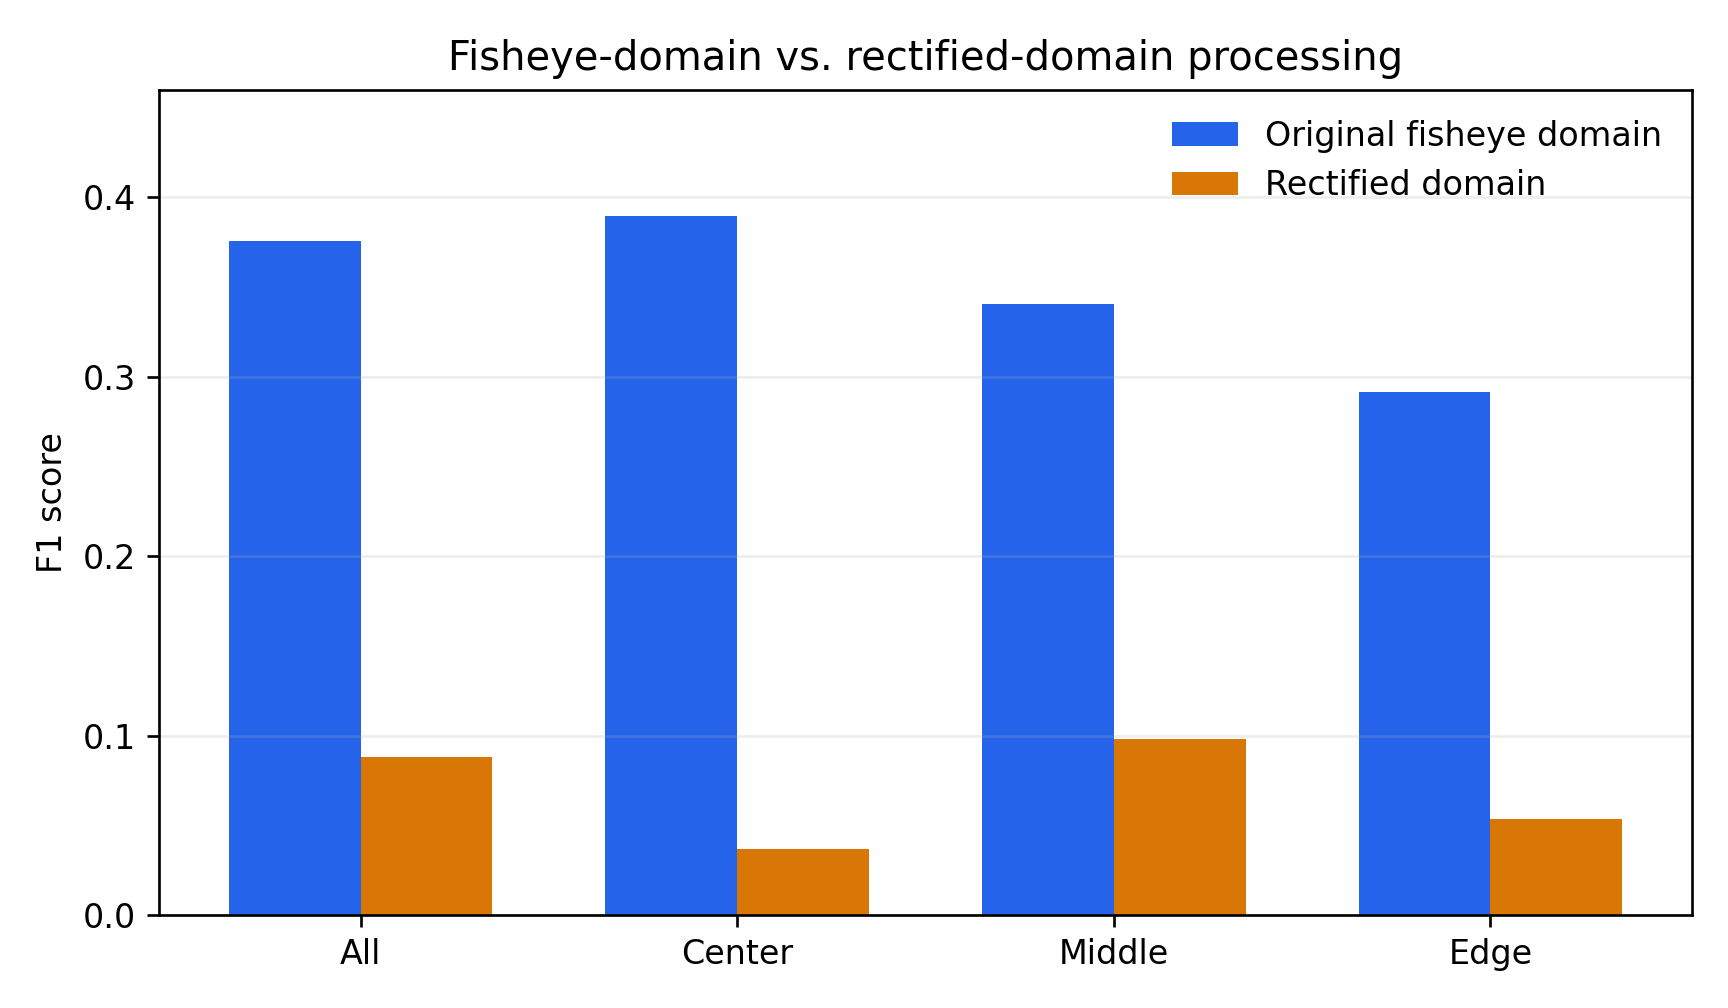
\includegraphics[width=\columnwidth]{../figures/route_comparison.png}
  \caption{\textbf{{\cjkfont 双路线} F1 {\cjkfont 对比。}} {\cjkfont 原始鱼眼域路线在多数方法上均优于先校正再反投影路线。}}
  \label{fig:route}
\end{figure}

\subsection{{\cjkfont 区域分析}}
\begin{table}[t]
\centering
\caption{{\cjkfont 区域} F1{\cjkfont 。边缘区域最能反映鱼眼畸变建模能力。}}
\label{tab:region}
\resizebox{\columnwidth}{!}{
\begin{tabular}{lccc}
\toprule
Method & Center & Middle & Edge\\
\midrule
YOLO-only & 0.3324 & 0.2811 & 0.2283\\
FisheyeMotionNet & 0.3950 & 0.2970 & 0.1340\\
UncertaintyFusion & 0.3953 & 0.2956 & 0.1300\\
\textbf{Full} & 0.3898 & \textbf{0.3404} & \textbf{0.2916}\\
Rectified Full & 0.0368 & 0.0980 & 0.0536\\
\bottomrule
\end{tabular}}
\end{table}

{\cjkfont 区域结果显示，完整模型对边缘区域的提升最明显。单体} FisheyeMotionNet {\cjkfont 的边缘} F1 {\cjkfont 为} 0.1340{\cjkfont ，而} Full {\cjkfont 模型达到} 0.2916{\cjkfont ，说明} SAM2.1 {\cjkfont 细化、}YOLO {\cjkfont 框提示和多源融合对畸变强烈区域具有互补作用。相比之下，校正域} Full {\cjkfont 在中心、中间、边缘均明显较低，进一步支持原始鱼眼域处理的选择。}

\subsection{{\cjkfont 消融分析}}
\begin{table}[t]
\centering
\caption{{\cjkfont 鱼眼域模块消融。数值为测试集全图} F1 {\cjkfont 和边缘} F1{\cjkfont 。}}
\label{tab:ablation}
\resizebox{\columnwidth}{!}{
\begin{tabular}{lcc}
\toprule
Variant & All F1 & Edge F1\\
\midrule
Full & 0.3758 & 0.2916\\
w/o RAFT & \textbf{0.3878} & 0.1646\\
w/o geometry & 0.3851 & 0.2032\\
w/o edge & 0.3617 & 0.1224\\
w/o DINO & 0.3225 & 0.1034\\
w/o YOLO & 0.0132 & 0.0000\\
\bottomrule
\end{tabular}}
\end{table}

{\cjkfont 消融结果揭示了几个有意义的现象。首先，}w/o RAFT {\cjkfont 和} w/o geometry {\cjkfont 的全图} F1 {\cjkfont 略高于} Full{\cjkfont ，但边缘} F1 {\cjkfont 明显下降，说明全图平均值会被中心和中间区域主导，而边缘区域更依赖运动与几何证据。其次，去除} DINOv2 {\cjkfont 后边缘} F1 {\cjkfont 从} 0.2916 {\cjkfont 降至} 0.1034{\cjkfont ，表明语义变化对困难区域有明显帮助。最后，}w/o YOLO {\cjkfont 几乎失效，说明在本数据规模下，实例先验仍是稳定召回运动目标的关键。}

\begin{figure}[t]
  \centering
  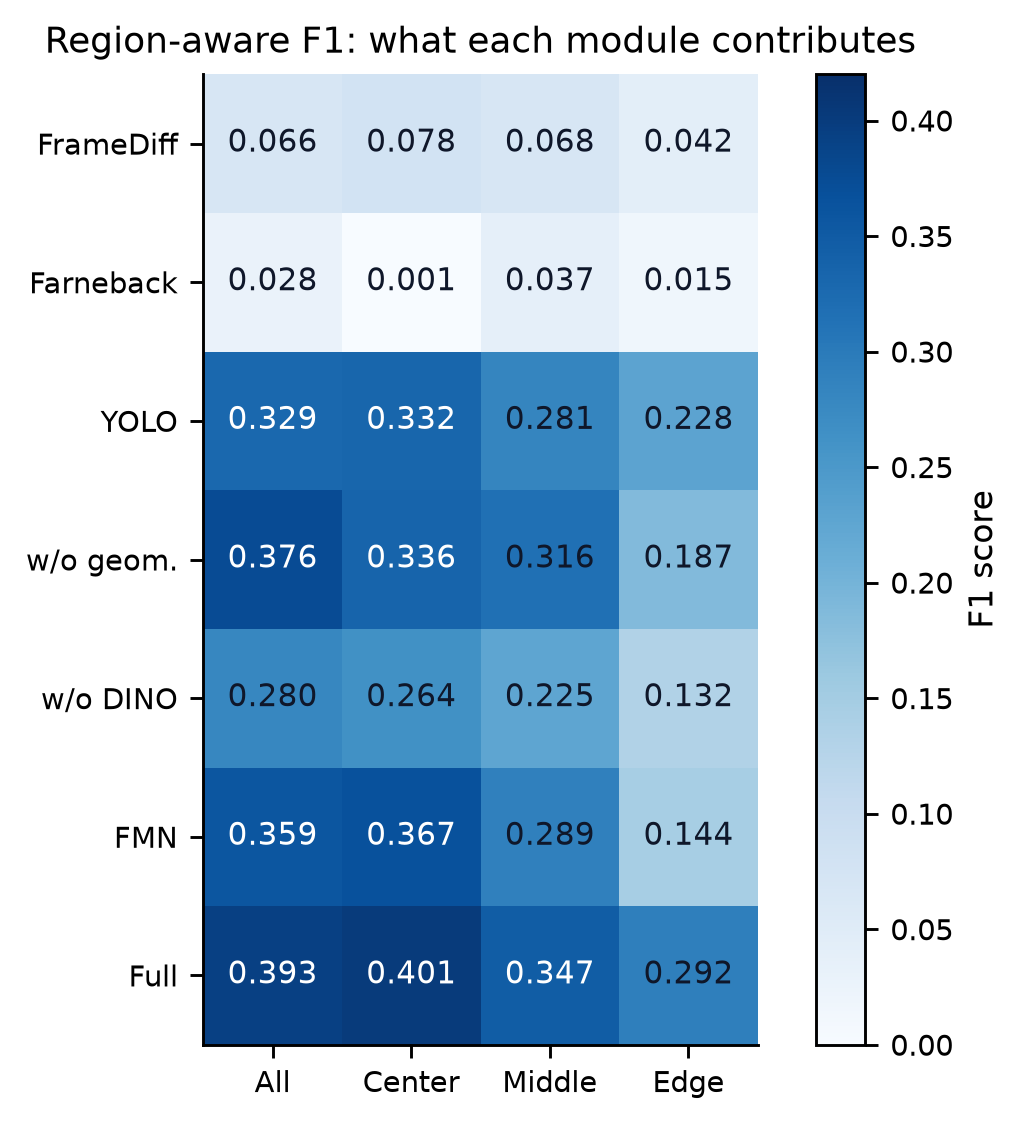
\includegraphics[width=\columnwidth]{../figures/ablation_region_matrix.png}
  \caption{\textbf{{\cjkfont 区域感知消融矩阵。}} {\cjkfont 行为方法或去模块版本，列为全图、中心、中间和边缘} F1{\cjkfont 。}}
  \label{fig:ablation}
\end{figure}

\section{{\cjkfont 定性结果与失败模式}}
{\cjkfont 图}~\ref{fig:qualitative} {\cjkfont 展示了代表性样本的当前帧、}GT{\cjkfont 、预测和误差图。模型通常能捕获车辆、行人和靠近边缘的运动目标；主要失败来自三类情况：大面积车体反光导致} FP{\cjkfont ，远处小目标或细长行人导致} FN{\cjkfont ，边缘区域反投影和插值误差导致校正路线掩膜破碎。}

\begin{figure*}[t]
  \centering
  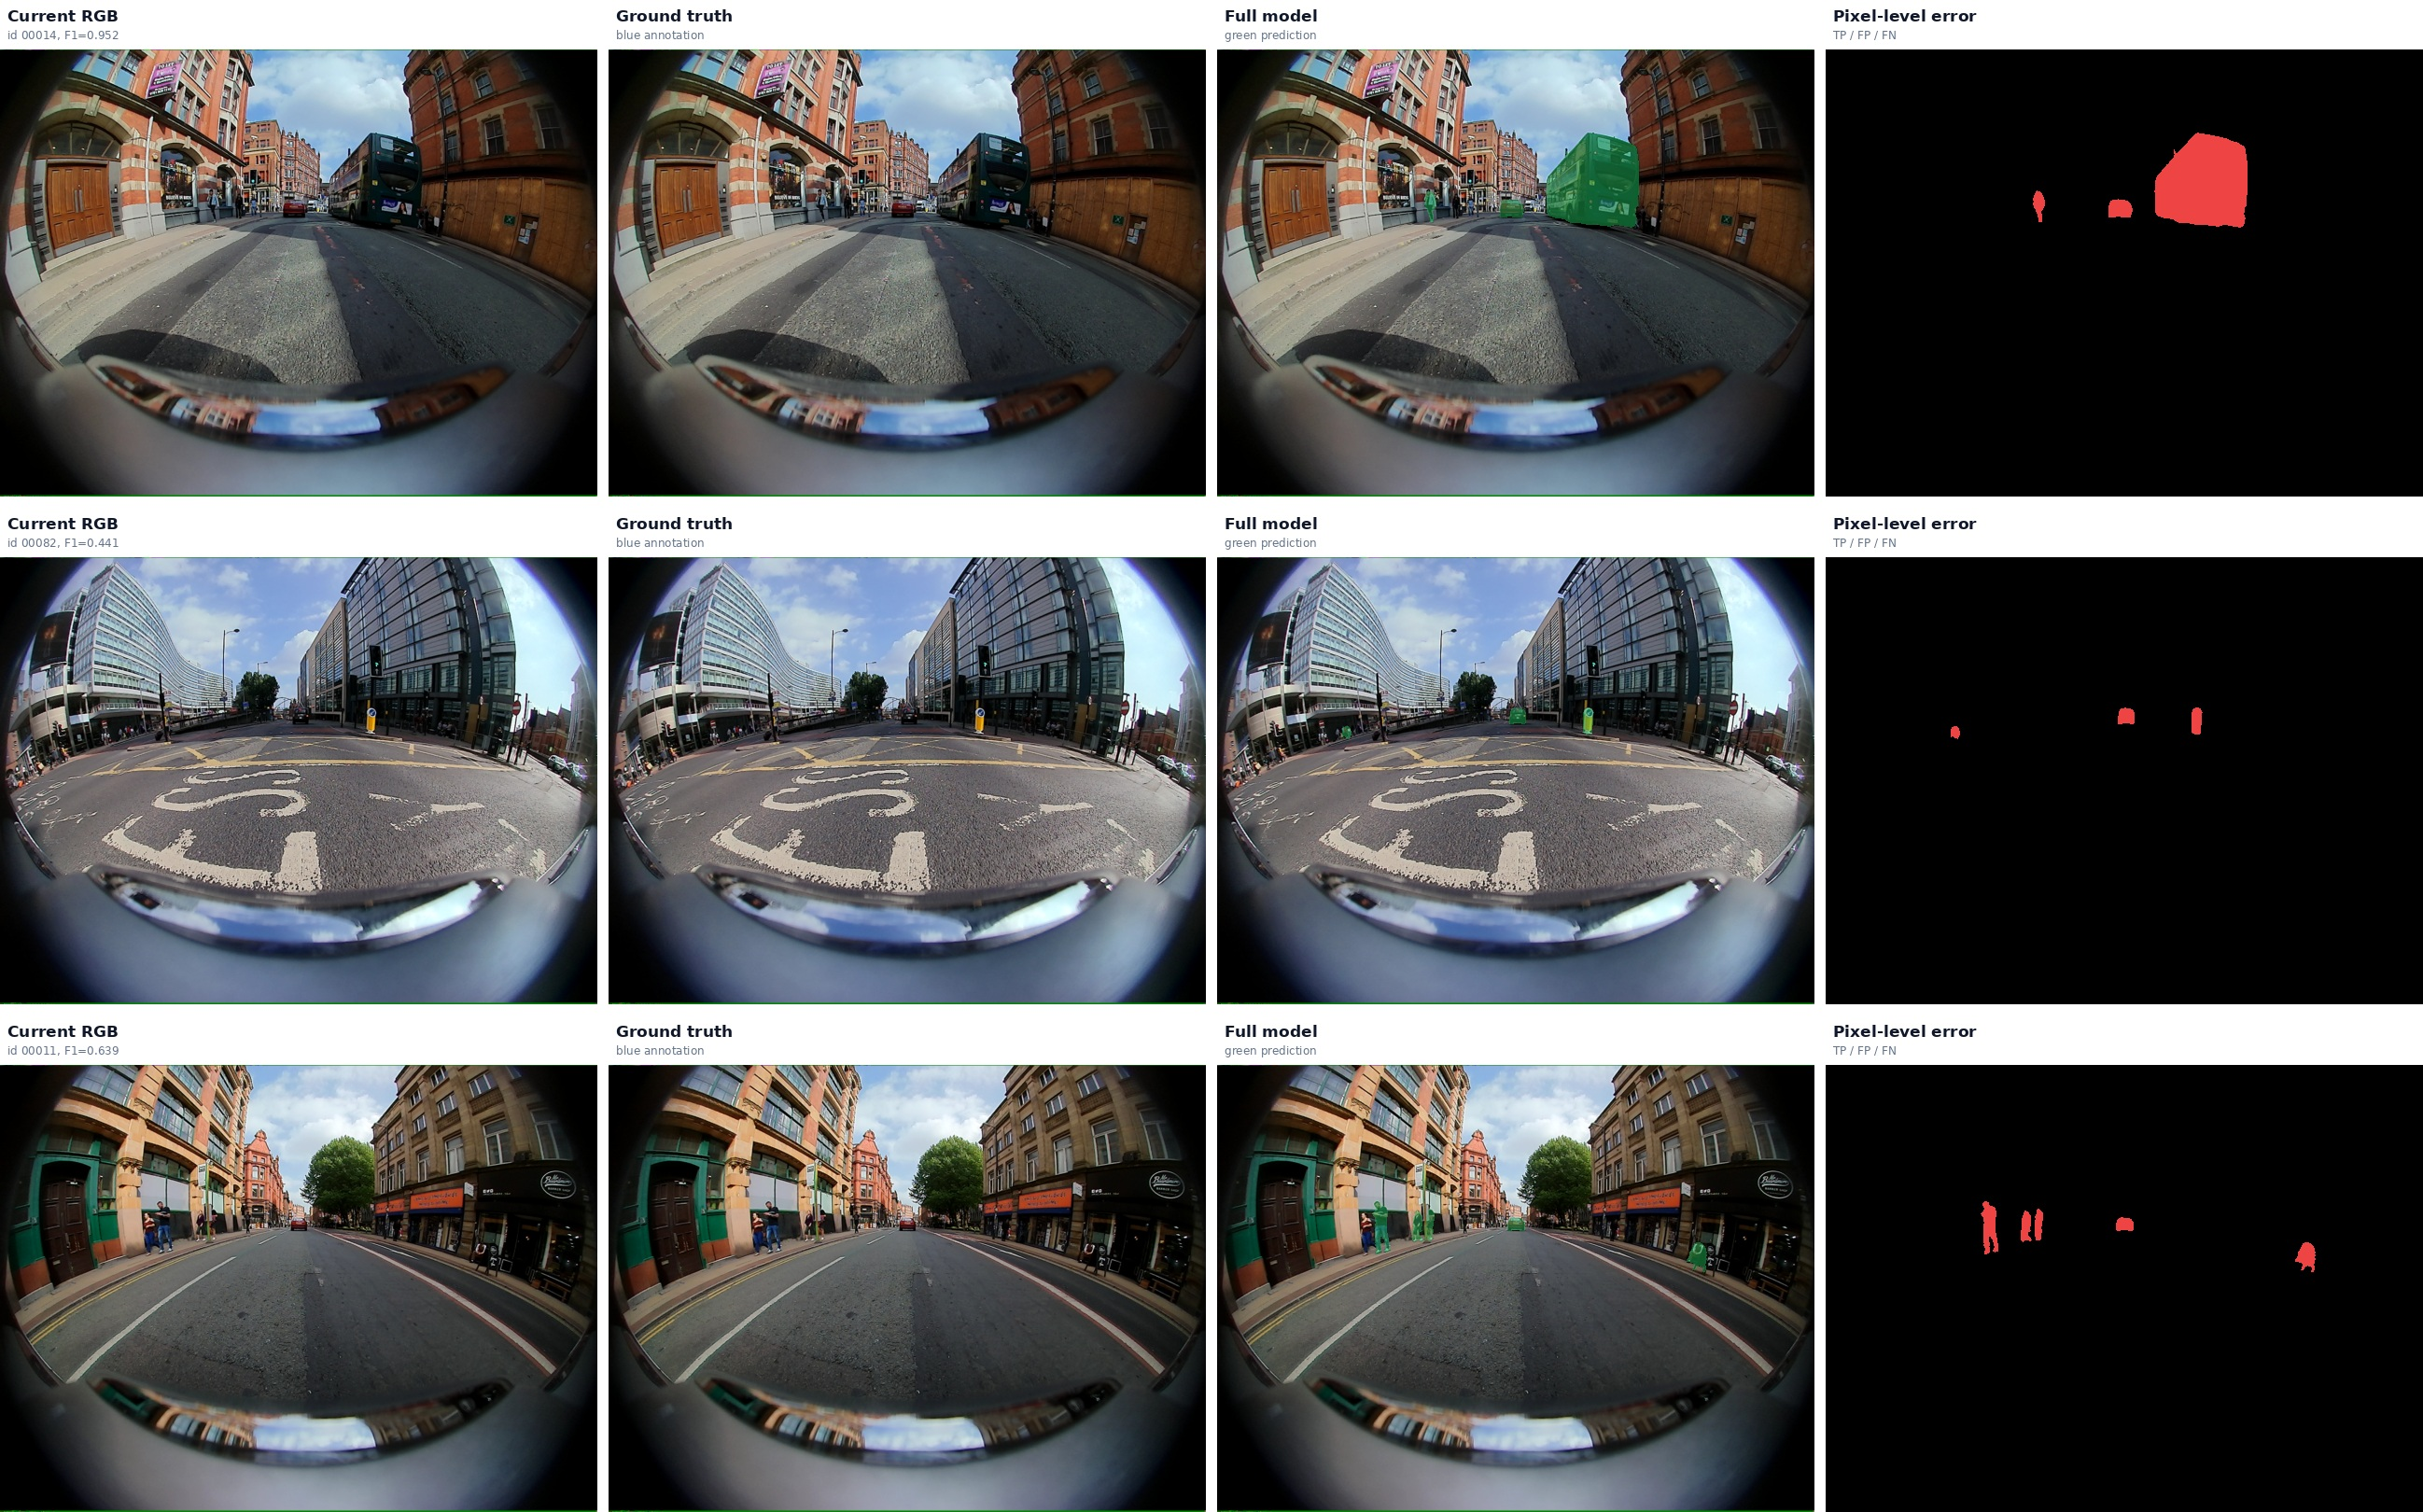
\includegraphics[width=\textwidth]{../figures/qualitative_comparison.jpg}
  \caption{\textbf{{\cjkfont 定性比较。}} {\cjkfont 每行展示一个测试样本，包含当前帧、}GT{\cjkfont 、}Full {\cjkfont 模型预测和像素级误差。}}
  \label{fig:qualitative}
\end{figure*}

\begin{figure}[t]
  \centering
  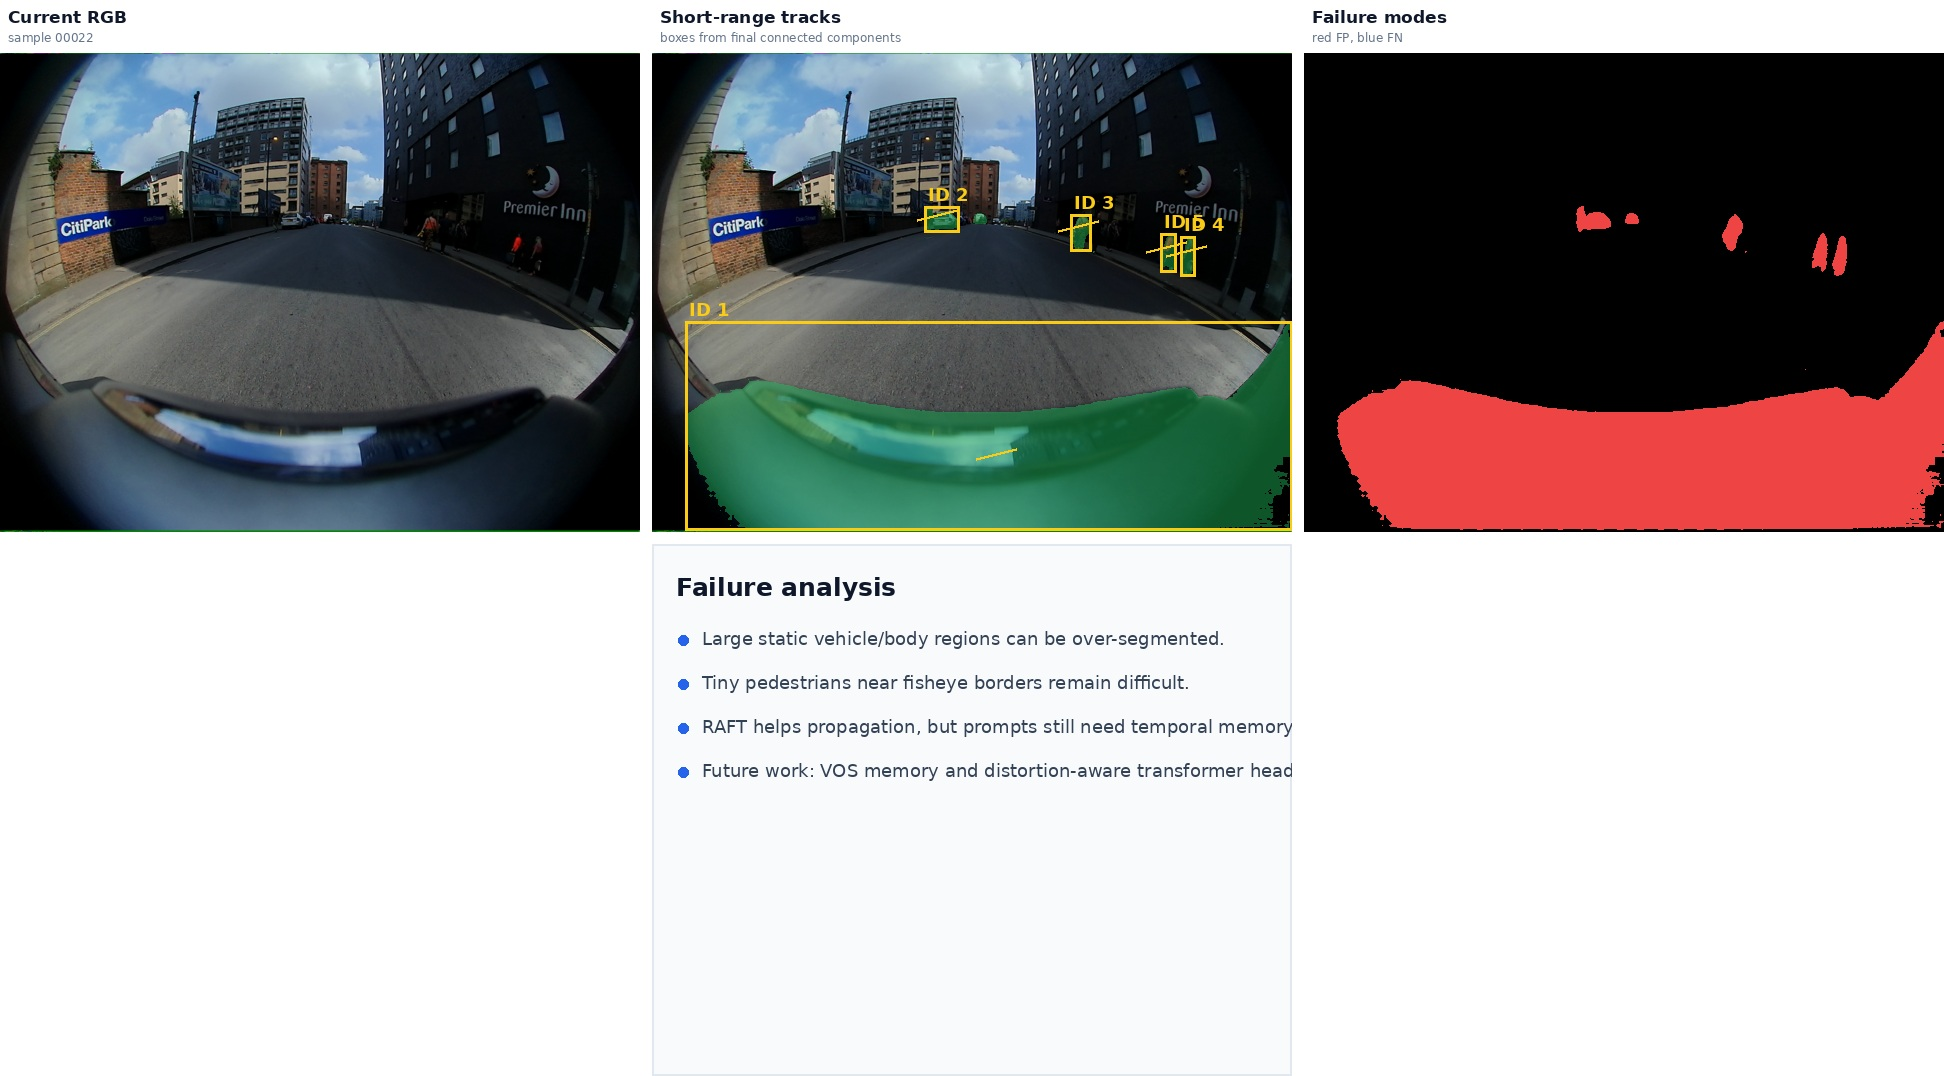
\includegraphics[width=\columnwidth]{../figures/tracking_failure_panel.jpg}
  \caption{\textbf{{\cjkfont 短时跟踪与失败分析。}} {\cjkfont 黄色框来自最终连通区域；误差图展示大面积} FP {\cjkfont 与小目标} FN{\cjkfont 。}}
  \label{fig:failure}
\end{figure}

\section{{\cjkfont 讨论}}
{\cjkfont 实验给出两个重要结论。第一，鱼眼运动分割的瓶颈不是单个模型是否足够强，而是证据之间如何约束。}YOLO-only {\cjkfont 能提供高召回但缺少运动性；}RAFT-only {\cjkfont 能提供运动但缺少实例和语义；}SAM2-FrameDiff {\cjkfont 受} prompt {\cjkfont 质量限制。第二，前置校正并非天然更优。校正能让图像局部更接近针孔视角，但也会改变纹理、边界和} mask {\cjkfont 对齐方式；当最终评估仍在鱼眼} GT {\cjkfont 上进行时，反投影误差会直接损害像素级指标。}

\section{{\cjkfont 局限与未来工作}}
{\cjkfont 当前数据规模较小，测试集只有} 19 {\cjkfont 个样本，结论仍需在更多天气、光照和相机型号上验证。其次，跟踪评估主要是短时关联，尚未覆盖} IDF1{\cjkfont 、}HOTA {\cjkfont 或长时遮挡恢复。第三，}Full {\cjkfont 模型对} YOLO {\cjkfont 先验依赖较强，}w/o YOLO {\cjkfont 消融几乎失效。后续工作可引入长视频记忆网络、}DINO/SAM {\cjkfont 伪标签扩增、畸变感知} transformer decoder{\cjkfont ，以及联合优化校正域和鱼眼域的一致性约束。}

\section{{\cjkfont 结论}}
{\cjkfont 本文完成了一个可复现的鱼眼视频运动区域抽象系统。实验表明，在本数据集和当前实现下，直接在原始鱼眼域处理并显式加入几何编码，是优于先校正再反投影的路线。完整模型在综合} F1{\cjkfont 、召回率和边缘区域} F1 {\cjkfont 上均显著优于传统} baseline{\cjkfont ，证明多源深度证据融合是处理鱼眼运动分割问题的有效方向。}

\bibliographystyle{plain}
\bibliography{references}

\end{document}
